% Tento soubor nahraďte vlastním souborem s přílohami (nadpisy níže jsou pouze pro příklad)

% Pro kompilaci po částech (viz projekt.tex), nutno odkomentovat a upravit
%\documentclass[../projekt.tex]{subfiles}
%\begin{document}

\chapter{RQT Graf hardwarových uzlů a jejich rozhraní}

\begin{figure}[h!]
	\centering
	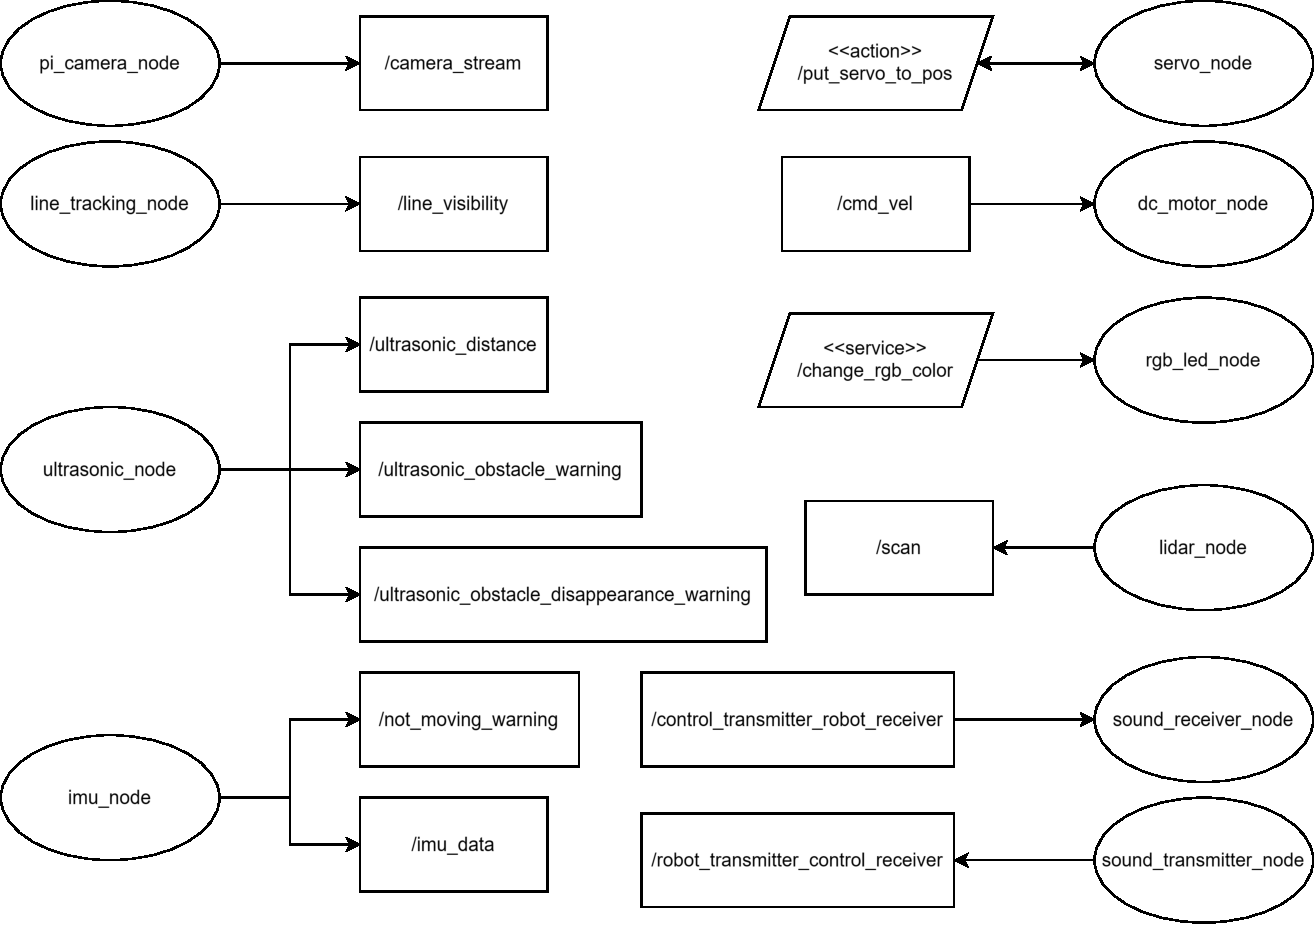
\includegraphics[scale=0.65]{obrazky-figures/hardware_nodes.pdf}
	\caption{RQT Graf hardwarových uzlů a jejich rozhraní}
	\label{}
\end{figure}

\chapter{RQT Graph řídícího systému}

\begin{figure}[h!]
	\centering
	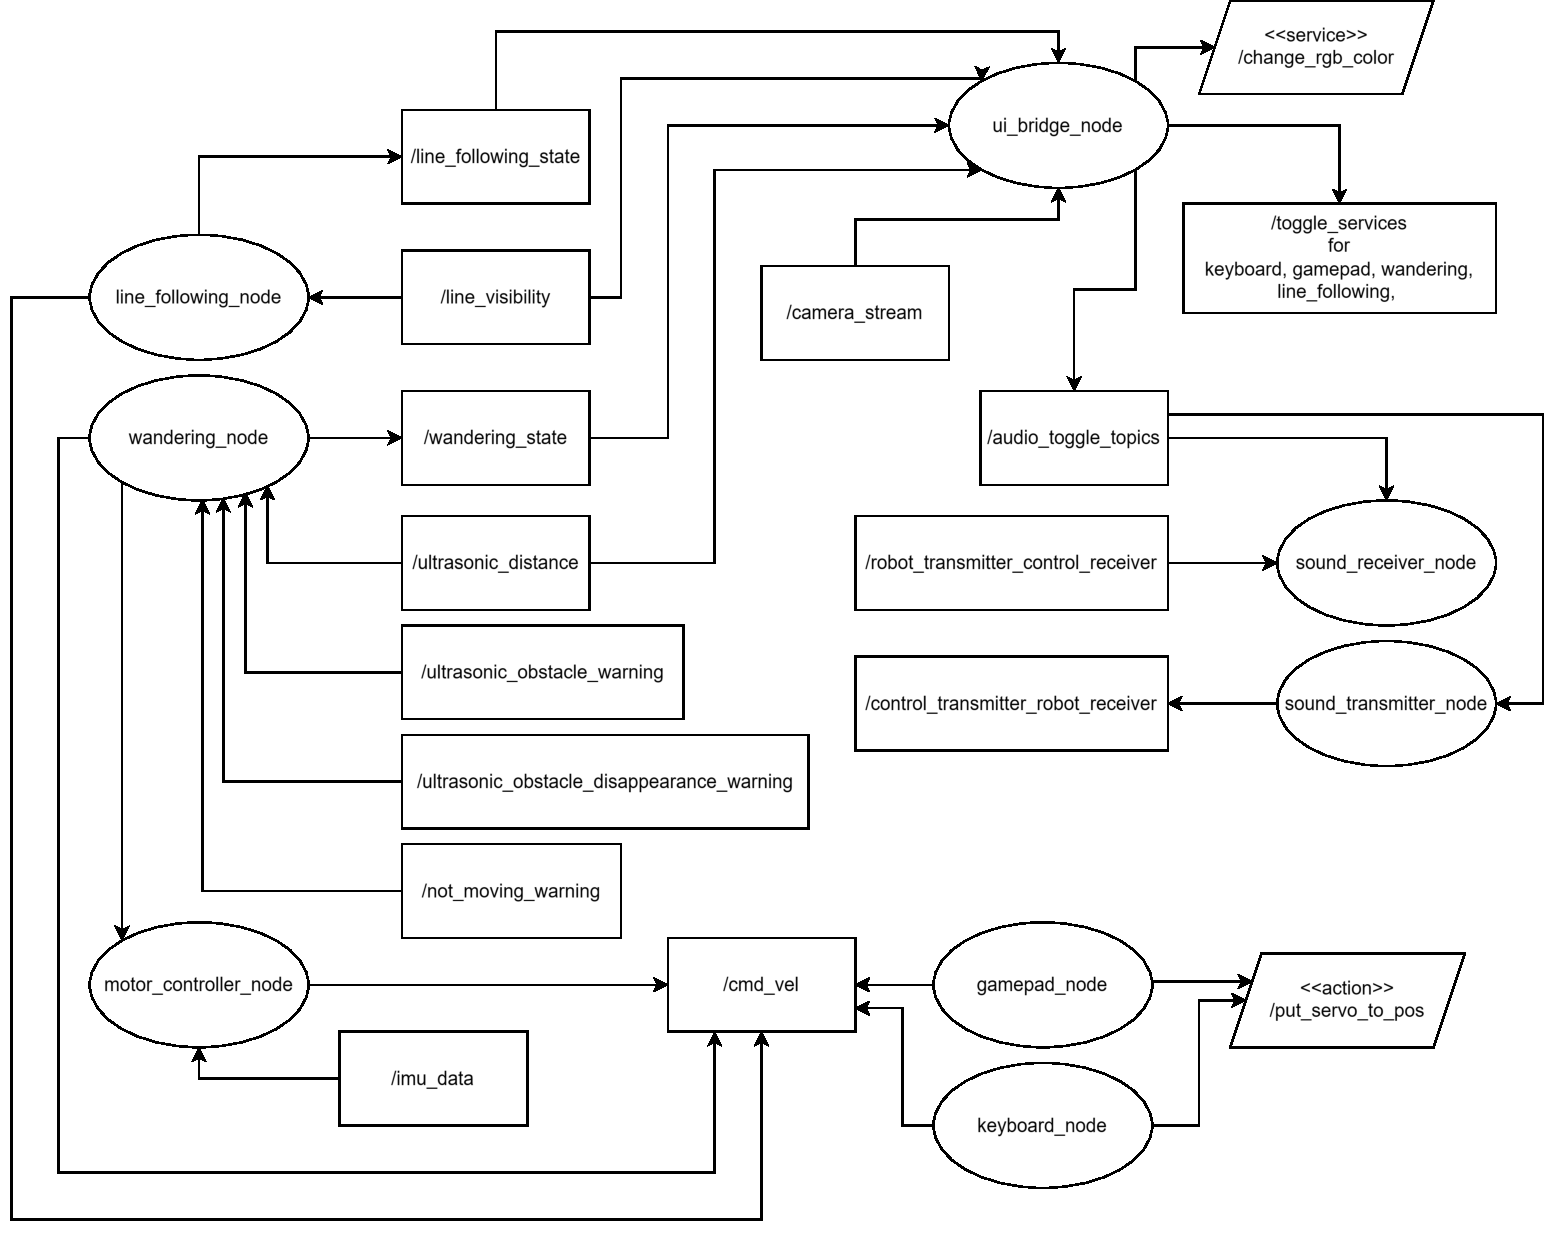
\includegraphics[scale=0.55]{obrazky-figures/controller_nodes.pdf}
	\caption{RQT Graph řídícího systému}
	\label{}
\end{figure}

% Pro kompilaci po částech (viz projekt.tex) nutno odkomentovat
%\end{document}
